\section{Analysis}

\subsection{Analytic treatment}

\begin{figure*}
\begin{centering}
\includegraphics[width=\textwidth]{lumpedModel.pdf}
\par\end{centering}
\caption{Lumped element model of the qubit and measurement circuit. a) The circuit is a ladder of alternating coupling capacitors and shunt resonators to ground. The only path by which energy can leave the system is through the finite internal quality factor $Q_F$ of the filter, as indicated by the red arrow. At the qubit frequency, the impedance of the coupling capacitors is greater than the impedance of the resonators. This means that most of the current flowing through eg. $C_g$ goes to ground through resonator $r$. b) To understand the quality factor of the resonator $Q_r$, we neglect the qubit which is assumed to be lossless. The damping of the resonator therefore comes entirely from the loss of the filter. Near resonance the filter impedance is a pure resistance.}
\label{Fig:lumpedModel}
\end{figure*}

In this section we derive an analytic expression for the $\kappa_r T_1$ product in the filtered measurement system.
We start from the definition of the quality factor for the qubit and, through standard circuit analysis, relate it to the quality factor of the filter.
We will find that the relation involves the ratio of the qubit and filter voltages, which we compute using voltage division.
An alternative method is to compute the complex admittance $Y_e$ presented to the qubit by the measurement circuit, and find the qubit $T_1$ using $T_1 = C_q / \Re Y(\omega_q)$ \cite{Esteve:dissipation1986}.
The approach used here should give the reader a more intuitive understanding of how the filter works.

An equivalent lumped model for the circuit is shown in Fig.\,\ref{Fig:lumpedModel}\,a.
We begin by writing down the definition of the quality factor of the qubit: \begin{equation}
Q_q \equiv \frac{\textrm{energy stored in qubit}}{\textrm{energy lost per radian of qubit oscillation}}. \label{eq:Q_qDefinition} \end{equation}
The energy lost per radian of oscillation can be re-expressed in terms of the qubit frequency and the power loss \begin{equation}
\textrm{energy loss per radian} = \frac{dE}{d\textrm{rad}} = \frac{dE}{dt} \frac{dt}{d\textrm{rad}} = \frac{P}{\omega_q} \label{eq:lossConversion} \end{equation}
where $P$ is the power loss and $\omega_q$ is the qubit oscillation frequency. Substituting Eq.\,(\ref{eq:lossConversion}) into Eq.\,(\ref{eq:Q_qDefinition}) gives \begin{equation}
Q_q = \frac{E_q \omega_q}{P} \label{eq:Q_qPower} \end{equation}
where here $E_q$ denotes the energy stored in the qubit.

If we assume that the circuit elements are lossless, then the only channel by which energy can leave the system is through the filter's coupling to the external measurement circuitry. The energy lost this way is characterized by the quality factor of the filter $Q_F$ \begin{equation}
Q_F \equiv \frac{\textrm{energy stored in filter}}{\textrm{energy lost per radian of filter oscillation}} = \frac{E_F \omega_F}{P} \label{eq:Q_FDefinition} \end{equation}
where here the second equality follows from the same reasoning that lead to Eq.\,(\ref{eq:Q_qPower}). Setting the power loss in Eq.\,(\ref{eq:Q_qPower}) equal to the power loss in Eq.\,(\ref{eq:Q_FDefinition}) gives \begin{equation}
Q_q = Q_F \frac{E_q \omega_q}{E_F \omega_F} = Q_F \frac{\omega_q}{\omega_F} \frac{C_q}{C_F} \left| \frac{V_q}{V_F}\right|^2 \label{eq:Q_qVoltage} \end{equation}
where we have taken $E_q = \frac{1}{2}C_q \left| V_q \right|^2$ and $E_F = \frac{1}{2} C_F \left| V_F \right|^2$, and $V_q$ and $V_F$ are the voltage amplitudes at the qubit and filter as shown in Fig.\,\ref{Fig:lumpedModel}\,a.

To compute the ratio $V_q/V_F$ we use voltage division. The analysis is based on the crucial observation that to compute the damping of the qubit we must analyse the circuit \emph{at the qubit frequency}. Because the qubit is off resonance from the measurement resonator and the coupling between the qubit and resonator is weak, the measurement resonator's impedance $Z_r$ is lower than the impedance of the coupling capacitor, ie. $Z_r \ll Z_g$. By similar reasoning $Z_r \ll Z_{\kappa}$. Therefore, with voltage $V_q$ across the qubit, we have a current $I_g = V_q / Z_g$ flowing through $C_g$ (see Fig.\,\ref{Fig:lumpedModel}\,a) and most of that current goes to ground through the resonator. This gives $V_r = I_g Z_r = V_q Z_r/Z_g$. Using similar arguments to work through the next stage of the circuit we arrive at \begin{equation}
\frac{V_q}{V_F} = \frac{Z_g Z_{\kappa}}{Z_r Z_F}. \label{eq:V_qOverV_F} \end{equation}
Note the shunt impedances in the denominator and the coupling impedances in the numerator.

Next we compute $Z_r$ and $Z_F$ in terms of their characteristic resonance impedances. The impedance of a lossless, parallel, single pole resonance is \begin{equation}
\frac{1}{Z} = i \omega C + \frac{1}{i \omega L} = \frac{i}{Z^0} \frac{2\delta x + \delta x^2}{1 + \delta x} \approx \frac{i 2 \delta x}{Z^0} \label{eq:resonanceImpedance} \end{equation}
where $\delta x \equiv (\omega - \omega_r)/\omega_r$, $\omega_r$ is the resonance frequency, and $Z^0$ is the characteristic impedance of the resonance ($Z^0 = \sqrt{L/C}$ for a parallel LC resonance). Inserting Eq.\,(\ref{eq:resonanceImpedance}) into Eq.\,(\ref{eq:V_qOverV_F}) we get \begin{equation}
\left| \frac{V_q}{V_F} \right| = \frac{\left| Z_g \right| \left| Z_{\kappa} \right|}{Z_r^0 Z_F^0} \left( \frac{2\delta x + \delta x^2}{1 + \delta x} \right)^2 \label{eq:VqOverV_F_2} \end{equation}
where here $\delta_x \equiv (\omega_q - \omega_r)/\omega_r$, $\omega_r$ is the measurement resonator frequency, and we assume the measurement resonator is on resonance with the filter. Inserting Eq.\,(\ref{eq:VqOverV_F_2}) into Eq.\,(\ref{eq:Q_qVoltage}) yields \begin{equation}
Q_q = Q_F \frac{\omega_q}{\omega_r} \frac{C_q}{C_F} \left( \frac{\left| Z_g \right| \left| Z_{\kappa} \right|}{Z_r^0 Z_F^0} \right)^2 \left( \frac{2\delta x + \delta x^2}{1 + \delta x } \right)^4. \label{eq:Q_qZ} \end{equation}

Equation (\ref{eq:Q_qZ}) expresses $Q_q$ in terms of the impedances of the couplers. While this can in principle be used as a design formula, it would be more convenient to replace the information contained in $Z_{\kappa}$ with an expression involving $Q_r$. To do this we consider the circuit at measurement frequency. With the measurement resonator and filter assumed to be on resonance, the filter impedance is nearly a pure resistance $R_F = Q_F Z_F^0$, as indicated in Fig.\,\ref{Fig:lumpedModel}\,b. As we assume the qubit is lossless, $R_F$ sets $Q_r$. Following reasoning similar to what lead to Eq.\,(\ref{eq:Q_qZ}) we find \begin{equation}
Q_r = \frac{\left| Z_{\kappa} \right|^2}{R_F Z_r^0} = \frac{\left| Z_{\kappa} \right|^2}{Q_F Z_F^0 Z_r^0}. \label{eq:Q_r} \end{equation}
Substituting Eq.\,(\ref{eq:Q_r}) into Eq.\,(\ref{eq:Q_qZ}) yields \begin{equation}
Q_q = Q_r Q_F^2 \left( \frac{C_q}{C_g} \right)^2 \left( \frac{Z_q^0}{Z_r^0} \right) \left( \frac{2\delta x + \delta x^2}{1 + \delta_x} \right)^4 \end{equation}
and using $Q_r = \omega_r \kappa_r$ and $Q_q = \omega_q T_1$ we find \begin{equation}
\kappa_r T_1 = Q_F^2 \left( \frac{\omega_r}{\omega_q} \right) \left( \frac{C_q}{C_g} \right)^2 \left( \frac{Z_q^0}{Z_r^0} \right) \left( \frac{2\delta x + \delta x^2}{1 + \delta x} \right)^4. \label{eq:kappa_rT_1_circuit} \end{equation}
Equation (\ref{eq:kappa_rT_1_circuit}) is our basic result giving the $\kappa_r T_1$ product for a filtered measurement system. As it expresses the product in terms of hardware parameters it is most useful when choosing values for the actual hardware and for constructing numerical simulations in circuit modelling programs.

In practice the resonant circuits are implemented as distributed transmission line resonators. In this case it is convenient to eliminate the characteristic resonance impedances in favor of the characteristic impedance of the line. For a $\lambda/4$ transmission line resonator, the resonance $Z^0$ impedance is related to the line impedance $Z_0$ by \cite{Pozar:microwaveEngineering2009} \begin{equation}
Z^0 = (4/\pi)Z_0 \end{equation}
which turns Eq.\,(\ref{eq:kappa_rT_1_circuit}) into \begin{equation}
\kappa_r T_1 = \frac{\pi}{4} Q_F^2 \left( \frac{\omega_r}{\omega_q} \right) \left( \frac{C_q}{C_g} \right)^2 \left( \frac{Z_q^0}{Z_0} \right) \left( \frac{2\delta x + \delta x^2}{1 + \delta x} \right)^4. \label{eq:kappa_rT1_lambda4} \end{equation}
We used Eq.\,(\ref{eq:kappa_rT1_lambda4}) as our design formula.

Equation (\ref{eq:kappa_rT_1_circuit}) expresses $\kappa_r T_1$ in terms of circuit hardware parameters. For an equation expressed in terms of implementation-independent parameters, we need to eliminate $C_g$ in favor of a coupling strength.
As derived in \citeinternaltype \citeinternalref{qubitTheory}, the equation which does this is \begin{equation}
g_e = \frac{1}{2}\frac{C_g}{\sqrt{C_q C_r}} \hbar \sqrt{\omega_q \omega_r}. \end{equation}
The subscript $e$ reminds us that this coupling strength has dimensions of energy. It is convenient to work with a coupling strength which has dimensions of (angular) frequency \begin{equation}
g \equiv \frac{g_e}{\hbar} = \frac{1}{2}\frac{C_g}{\sqrt{C_q C_r}} \sqrt{\omega_q \omega_r}. \label{eq:couplingStrength} \end{equation}
Using Eq.\,(\ref{eq:couplingStrength}) and keeping the leading order in $\delta x$ we can re-express Eq.\,(\ref{eq:kappa_rT_1_circuit}) as \begin{equation}
\kappa_r T_1 = \left( \frac{\Delta}{g} \right)^2 \left( \frac{\omega_r}{\omega_q} \right) \left( \frac{\Delta}{\omega_r / 2 Q_F} \right) ^2 \label{eq:kappa_rT_1} \end{equation}
where $\Delta \equiv \omega_q - \omega_r$.
The first factor, $\left( \Delta / g \right)^2$ is the $\kappa_r T_1$ product for a single pole (i.e. no filter) system.
The second factor is of order one.
The final factor is understood as as the isolation provided by the filter: $\omega_r / 2 Q_F$ is the half width at half max of the filter (recall that we assume $\omega_r = \omega_F$), so $\Delta / \left( \omega_r/2 Q_F \right)$ is the qubit-filter detuning in units of half-widths.
This factor substantially raises the $\kappa_r T_1$ product.
For $\omega_q=6\,\text{GHz}$, $\omega_r = 7\,\text{GHz}$, and $Q_F=30$ we find \begin{equation}
\left( \frac{\omega_r}{\omega_q} \right) \left( \frac{\Delta}{\omega_r / 2 Q_f} \right)^2 = 85, \end{equation}
almost two orders of magnitude improvement over the unfiltered case.